% background
% brief review of previous research (cite)
% reson why the research was undertaken
% Hypothesis
% explenation of techniques and why they ve been chosen
% objectives = what you hope to achieve
% brief reference to the main outcome

%$\ce{CdS_x Se_{1-x}/ZnS}$

% \begin{figure*}
%   \centering
%   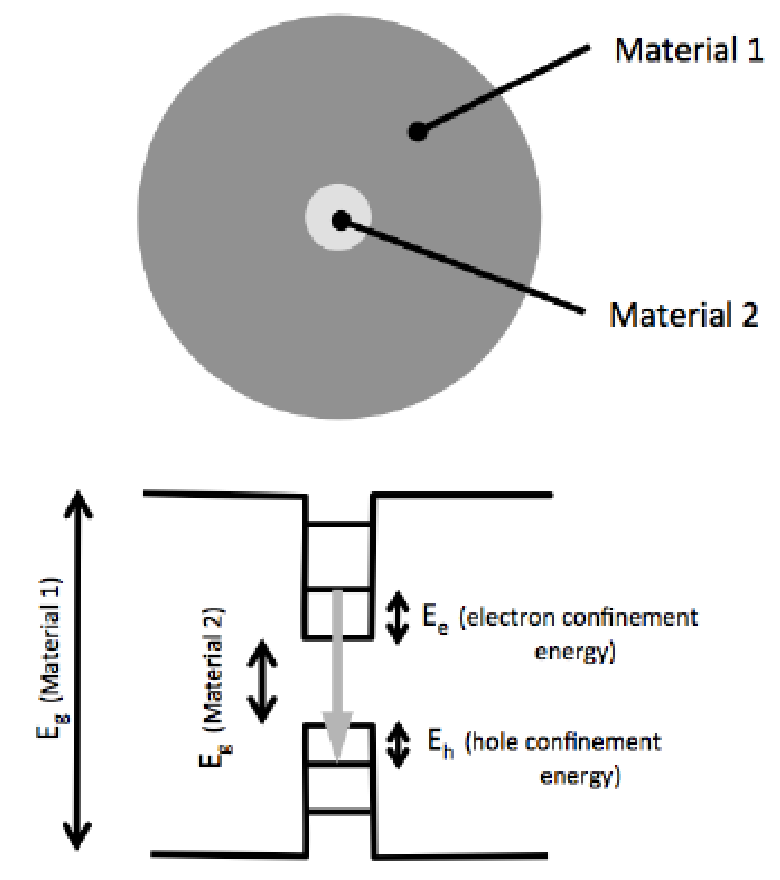
\includegraphics[width=0.35\textwidth]{graphics/QD.png}
%   \caption[width=0.4\textwidth]{\cite{instruction}.}
%   \label{fig:QD}
% \end{figure*}

\section{Introduction}
\label{sec:Introduction}

Nowadays electronics, both at the consumer market but also in the high tech industry and research is based on microelectronics.
High standards in quality and reproductability have to be implemented.
These standards can directly be linked with the manufacturing of nanostructures, which is what got to be analyzed in this report by using a photodector as an example.

Generally one can devide the manufactering of two-dimensional electronic components into two branches.
There is the top-down approach and the bottom-up approach which is used for our purpose.
The benefit here can be that less material is wasted as some of the elements used may be rare and or expensive this is an argumnet take into account to.

At the end, the produced working circuit is characterized optically and electronically. 
The finished photodector is based on a photoconductor architecture with gold contacts and a active layer of polycrystalline perovskite ($\ce{MAPbBr_3}$) with a bandgap of $\SI{2.2}{\eV}$.

In the following, the detailed manufactering process with the used materials and techniques is presented.

\subsection{Cleaning of the substate}
\label{sec:cleaning}

As a substrate glass is used, as it is heat and radiation resistant but also do not react with the very most of elements.
As the deposited active layers are expected to be only micrometers thick, any kind of impurity on the glass surface may interfere the quality and thus functionality of the device.
Therefore, several cleaning steps are introduced.
Firstly, some soap and water, then just water and then Aceton is used to clean the surface inside a ultrasonic bath.
To remove the agressive aceton, propanol is used and removed by a nitrogen flow from the surface.
This has the benefit, that eventually solved elements in the liquid do not stay on the surface as the liquid would evaporate.
At the very end, the glass is baked to remove condensated water.

\subsection{Photoresist Spincoating}
\label{sec:spincoating-resist}

In order to create the finestructured electronic wires on top of the surface, photolithography is used.
Therefore, a positive photoresist has to be deposited uniformly onto the glass surface.
As the photoresist material is sensitive to blue and UV light, the laboratory is luminated by yellow light only.

\begin{figure*}
    \centering
  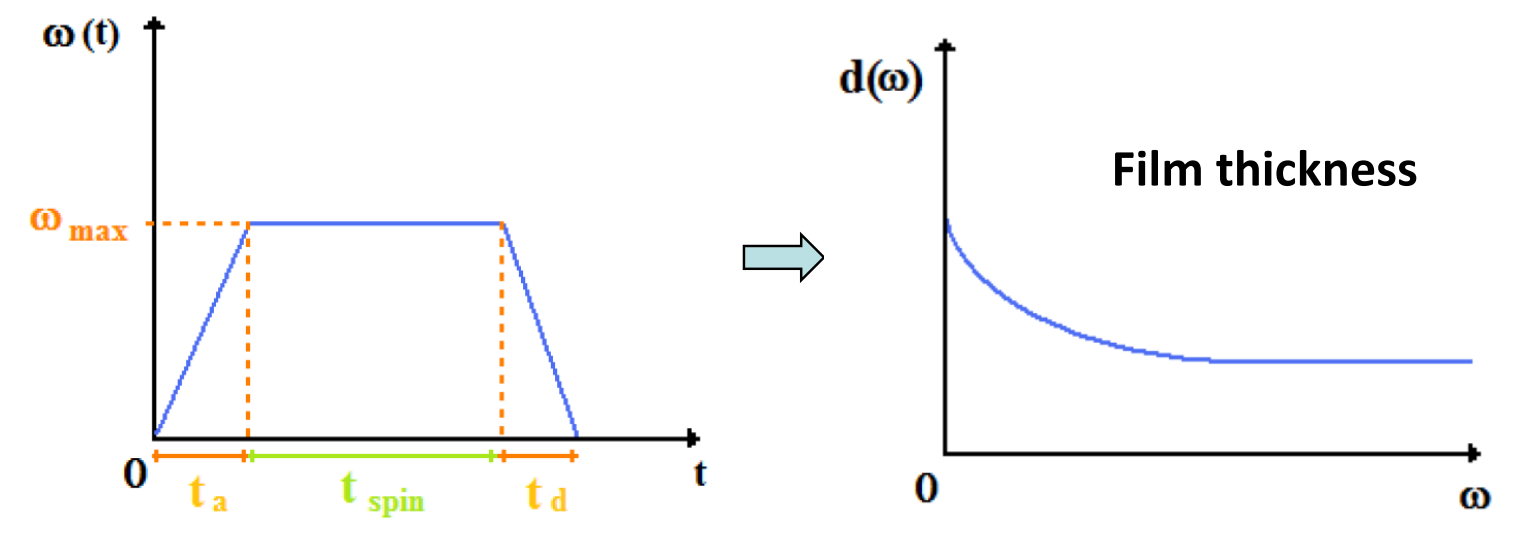
\includegraphics[width=0.7\textwidth]{graphics/spincoat.png}
  \caption[width=0.7\textwidth]{Impact of the free parameters of a spincoating procedure on the film thickness, in the time and frequency domain\cite{instruction}.}
  \label{fig:spincoat}
\end{figure*}

Spincoating can be used to deposit viscous solutions uniformly onto a surface by the centrifugal force, which is done here with the photoresist material.
To get a good result it is important to choose the rotating paremters well.
As we can see in figure \ref{fig:spincoat}, the rotating frequency has to be set high enought, whereas a arbitary increase do not change the film thickness anymore.
Nethertheless, the ramping and decleration time are parameters to set.
In this case, 4000rpm, $\SI{1}{\sec}$ of ramp and $\SI{60}{\sec}$ of dwell are set.
After deposition the sample is baked out to evporate the solvant of the photoresist.

\subsection{Photoresist writing}
\label{sec:writing}

The wished pattern of connection is exposed by UV light in this step.
As the positive photoresist exposed can be removed easily by a developer, the later evaporated gold can stick directly onto the glass surface.
In detail, a maschine called MicroWriter is used for this process. The wished pattern is projected by computer-controlled optics onto the surface.
Before doing this, it is important to set the focus onto the glass surface in high precision, as a missalignment has direct effects on the resolution of the structures edges.
The minimum feature size of the used device is about $\SI{1}{\micro\meter}$.

After the machine processed the sample is exposed a MF-319 developer for 45sec and dried later.
As mentioned above the wished pattern for the gold contacts is the free glass surface, now.

\subsection{Gold contacts}
\label{sec:evaporation}

By thermal evaporation inside an UHV chamber a uniform, thin layer of gold can be deposited onto the sample.
The material is choosen because of its high electric conductivity.

The so called lift-off can follow, where the stack of photoresist and with it the remaining gold on top can be dissolved from the glas. 
Ideally, only the gold contacts on the glass remain, as the gold is not attacked by the here used acetone.
The process needs around 4 hours.

\subsection{Perovskite deposition}
\label{sec:perovskite}

As the perovskite is dissolved in a liquid, the in section \ref{sec:spincoating-resist} mentioned spincoating tecnique can be used for deposition.
The only difference is, that the samples surface has to be roughted up with a plasma cleaner.
As the ionized atom cores or the free electrons are bombarding the surface, the surface increases and the deposited perovskite holds better on the surface.

In following, two different methods and thus samples are prepared. 
The first one is equivalent to the steps in section \ref{sec:spincoating-resist}, as the solvant is evaporated slowly by heating the sample.
For the second sample, the hardening of the solvant is done by adding an antisolvant, here Clorobenzene, onto the surface, while the spincoater is still spinning.
The idea of this procedure is, that the perovskite is not solvable in the antisolvant, but the solvant is, so that the perovskite is immideatly forsed to crystalize.
Both samples are baked out for 30min.

\subsection{Device characterization}
\label{sec:charact-intro}

The characterization of the sample has firstly the purpose to check the functionallily of the here produced photodetector.
Therefore the conductance of the sample, with and without light exposion is measured, using a low noise micro probe station.
A voltage bias in the range of $\SI{\pm 20}{\V }$ is applied.

The second purpose is to characterize the two different manufacturing approaches mentioned in section \ref{sec:perovskite}.
Therefore, not only the electronic measurement but also an optical analyzis under the microscope is used.





